\documentclass{article}
\usepackage{xcolor}
\usepackage{graphicx}
\usepackage{caption}
\usepackage{subcaption}
\usepackage[utf8]{inputenc}
\usepackage[T1]{fontenc}
\usepackage[francais]{babel}
\usepackage{hyperref}
\hypersetup{
colorlinks=true,
breaklinks=true,
urlcolor= blue,
linkcolor= black,
citecolor=black,
}
\usepackage{enumitem}
\usepackage{float}
\usepackage{pifont}

\addtolength{\textwidth}{3cm}
\addtolength{\oddsidemargin}{-1.5cm}


\begin{document}
%-----------------------------------------------------------------------
\hrule
\begin{center}
\Huge {\textsc{CULTUR'ADVISOR - Développement d'une plateforme}}
\end{center}
\hrule
\vspace{10mm}
\begin{center}
\Large \textsc{Master 2 IMIS \\ Année 2022-2023}
\end{center}
\vspace{15mm}
\begin{figure}[H]
\hspace{-10mm}

\includegraphics[scale = 1.7]{images/logo.png}
\end{figure}
\vspace{30mm}

\begin{center}
\vfill{\Large \textsc{ Présenté par : Barodine Anaël, Mbelek-Nouga Paul-Dubien, TESSIER Adrien, Ververke Xavier \\ Encadré par : Tandjaoui Rosa et Hakim Aoudia}}
\end{center}
\begin{figure}[H]
\hspace{-0mm}

\includegraphics[scale = 0.4]{images/logo_orleans.png}
\hspace{10mm}

\includegraphics[scale = 0.4]{images/logo1.png}
\hspace{10mm}
\includegraphics[scale = 0.15]{images/logo_dill.png}
\end{figure}
\newpage
%-----------------------------------------------------------------------
\vspace*{\stretch{1}}
\begin{center}
\Large\bfseries
\title -Remerciements
\end{center}
\hspace{4.5mm} 
Tout d'abord, nous tenons à remercier Rosa Tandjaoui, notre mentor, et Matthieu Exbrayat notre encadrant universitaire de nous avoir accompagnés et guidés pour ce projet.

Nous voulons aussi remercier toutes les personnes qui ont contribué au succès de ce projet et qui nous ont aidés lors de la rédaction de ce rapport.
\vspace*{\stretch{1}}
\newpage
%-----------------------------------------------------------------------
\tableofcontents
\newpage %aller a la page suivante
%-----------------------------------------------------------------------
\section{contexte du projet}
À la croisée de l’agenda culturel, du média, du magazine et du réseau social, CulturAdvisor est un espace de productions, de consultations et d’échanges autour de la culture. \\
En France, il n'existe pas de base de données regroupant l'ensemble des produits sulturels du territoire. Il existe bien de telles bases mais elles sont restreintes à de plus petites zons géographiques. Tout cela rend plus difficile pour le public de les découvrir. \\
L'objectif de l'entreprise est donc de faciliter l’accès à la culture en aidant les acteurs à trouver de nouveaux publics, améliorer leur visibilité, augmenter leur fréquentation et pour le public, à trouver l’expérience culturelle qui leur ressemble, leur correspond.


\section{organisation de l'équipe}
Afin de mener ce projet à bien, nous avons d'abord commencé par se répartir les différentes taches du projet qui sont de récupérer l'ensemble des données disponible, les uniformiser, en faire une base de données, puis pouvoir faire des requêtes sur ces données.\\
Nous avons utilisé Watsapp pour être en contact avec notre mentor.\\
Projet partagé sur GitHub.


\section{Projet}


\subsection{Mis en place du projet}
Premièrement, nous avons commencé par choisir un environnement de travail.\\
Nous avons choisit le langage Python et le framework Flask. (anael si tu sait comment bien l'expliquer)

\subsection{Création du serveur Flask}
(anael)

\subsection{Récupération des données}
Une fois le serveur Flask mis en place, il faut maintenant pouvoir récupérer les différentes données disponible.\\
Nous avons eu par notre mentor une liste d'API contenant des différents produits culturels à récupérer.\\
Nous avons commencer par analyser ces différentes base de données puis nous avons récupérer chaque colonne.\\
\begin{figure}[H]
\hspace{-25mm}
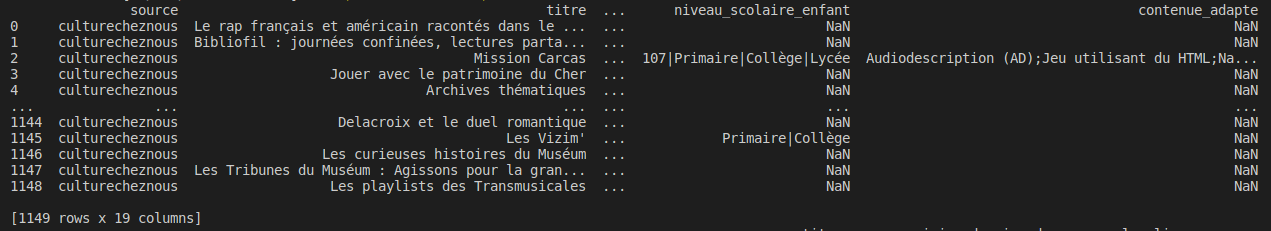
\includegraphics[scale = 0.44]{images/culturecheznous.png}
\caption{Dataframe contenant les données de culture chez nous}
\end{figure}
\begin{figure}[H]
\hspace{-25mm}
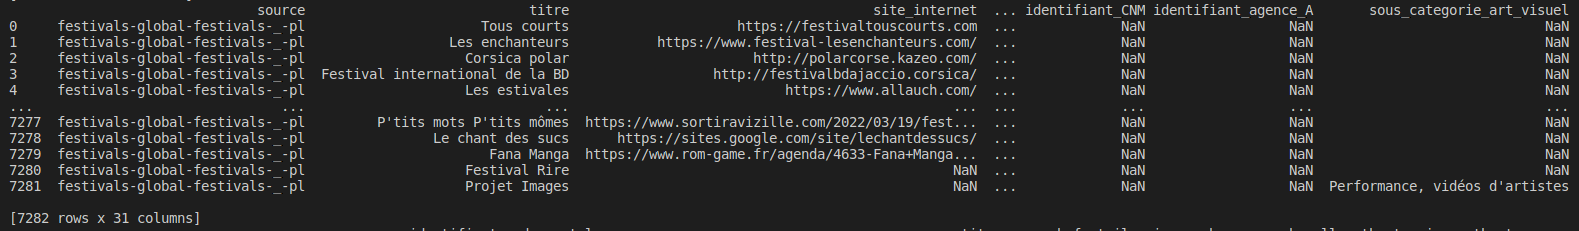
\includegraphics[scale = 0.354]{images/festivals.png}
\caption{Dataframe contenant les données des festivals en France}
\end{figure}

\subsection{Normalisation des données}
Après avoir récupérer ces données, nous avons du les normaliser.\\
Pour cela, nous avons utiliser un DataFrame afin de mettre tout les tableaux récolté dans un seul.\\
Pour commencer, on a regardé les colonne qui contenait les mêmes choses puis on a changer les noms de colonnes afin que chaque tableaux de données qui contenait les memes données ait le meme nom de colonnes afin qu'il soit normalisé.
\begin{figure}[H]
\hspace{-25mm}
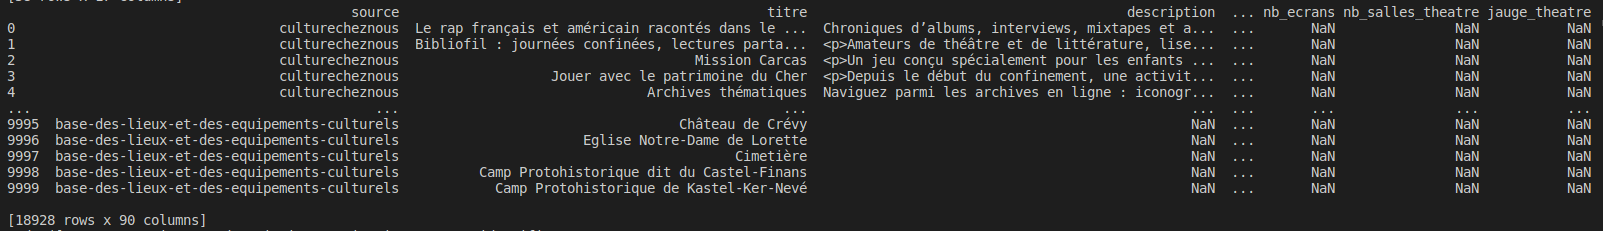
\includegraphics[scale = 0.35]{images/dataframe_final.png}
\caption{Dataframe contenant toutes les données après la normalisation}
\end{figure}

\subsection{Mise sous forme de base de données}
Nous avons par la suite fait des requêtes...

\subsection{Requêtes}
Pas encore fait ...

\section{Conclusion}
A écrire ...


\end{document}
